% !TEX encoding   = UTF8
% !TEX spellcheck = ru_RU
% !TEX root = ../seminars.tex

%%===========================================
\chapter{Технические детали: классы и прочее}
%%===========================================

%%====================================================
\section{Положение на плоскости. Класс \texttt{Vec2d}}
%%====================================================
Создадим небольшой вспомогательный класс \code{Vec2d} для~указания положения объекта на~плоскости. Позже мы сможем им воспользоваться при~рисовании двумерных фигур.

Заголовочный файл \code{lib/vec/vec2d.h} описывает данный класс, объявляет удобные операции над~его экземплярами.

\cppfile[firstline=4, lastline=13]{projects/lib/vec/vec2d.h}
\cpp`  // ...`
\cppfile[firstline=16, lastline=16]{projects/lib/vec/vec2d.h}
\cpp`// ...`
\cppfile[firstline=19, lastline=20]{projects/lib/vec/vec2d.h}
\cppfile[firstline=23, lastline=23]{projects/lib/vec/vec2d.h}

Загадочные имена параметров \code{lhs} и \code{rhs}, используемые при~перегрузке операторов, соответствуют сокращениям от~\textenglish{left hand side} (то есть слева от~оператора) и \textenglish{right hand side} (то есть справа от~оператора).

Реализацию методов разместим в~файле \code{lib/vec/vec2d.cpp}.

\cppfile[lastline=10]{projects/lib/vec/vec2d.cpp}
\cpp`// ...`
\cppfile[firstline=31, lastline=36]{projects/lib/vec/vec2d.cpp}
\cppfile[firstline=40, lastline=40]{projects/lib/vec/vec2d.cpp}

Добавьте остальные необходимые операторы самостоятельно.



%%=======================================
\section{Тесты для~класса \texttt{Vec2d}}
%%=======================================
Каким образом протестировать функционал нашего класса? Мы можем написать разнообразные выражения. Таким образом, мы охватим все возможные варианты его использования. На~этом этапе нас будет защищать сам компилятор, выдавая ошибки, если мы что-то не~реализовали или сделали это неправильным образом.

\begin{consolecode}
$ bin/vec
...
q + q      = {0, 2} [OK]
r + q      = {1, 1} [OK]
r += r     = {2, 0} [OK]
...
length(2 * s + 3 * p)     = 3.60555  [OK]
length(t)                 = 1.41421  [OK]
-----------
31 passed of 31 total
\end{consolecode}

Добавим файл \code{08/vec/main.cpp}. Сделаем набросок кода, чтобы получить вывод, подобный приведённому выше.

\cppfile[lastline=7]{projects/08/vec/main.cpp}
\cpp`// ...`
\cppfile[firstline=32, lastline=33]{projects/08/vec/main.cpp}
\cpp`  // ...`
\cppfile[firstline=55, lastline=66]{projects/08/vec/main.cpp}
\cpp`  // ...`
\cppfile[firstline=87, lastline=89]{projects/08/vec/main.cpp}

Тесты можно хранить в~векторе. Каждый элемент должен содержать выражение как строку (\code{std::string}), результат вычисления этого выражения (\code{Vec2d}) и ответ (\code{Vec2d}). Создадим для этого небольшую структуру.

\cppfile[firstline=9, lastline=14]{projects/08/vec/main.cpp}

Добавим реализацию операторов сравнения для~вектора на~плоскости, чтобы сравнивать результат с~ответом.

\cppfile[firstline=25, lastline=30]{projects/08/vec/main.cpp}

\noindent Нужно убедиться, что эти операторы верно запрограммированы, поскольку мы используем их для~проверки успешности прохождения тестов.

\cppfile[firstline=34, lastline=42]{projects/08/vec/main.cpp}

Добавим тесты, перебирая различные варианты, пытаясь <<сломать>> реализацию операций над~вектором \code{Vec2d}, найти выражения, которые могут не~сработать.

\cppfile[firstline=44, lastline=53]{projects/08/vec/main.cpp}

Каждый элемент вектора, имеющий тип \code{TestV}, мы инициализируем тройкой, например, \cppinline/{"r + r", r + r, {2, 0}}/. Однако, мы не~хотели бы дублировать выражение сначала в~строку, а затем как есть. По~этой причине мы добавили макрос, который получает такую пару из~обычного выражения (подобно тому, как это делали ранее, см.~страницу~\pageref{par:macro}).

\cppfile[firstline=23, lastline=23]{projects/08/vec/main.cpp}

По~аналогии, добавляем тесты для~функции \code{length()}.

\cppfile[firstline=68, lastline=85]{projects/08/vec/main.cpp}

К~сожалению, здесь мы не~можем использовать тип \code{TestV}. Нужно хранить не~пару векторов, а просто пару чисел. Для~этой цели придётся создать ещё один тип.

\cppfile[firstline=16, lastline=21]{projects/08/vec/main.cpp}

Далее мы познакомимся с~шаблонами, которые изящно решают эту проблему, подобно тому, как с~этой задачей справляется контейнер \code{std::vector}.



%%=================================
\section{Проект для \texttt{CMake}}
%%=================================
Скопируем проект, который создавали для~калькулятора (см.~страницу~\pageref{sect:calcproj}) и слегка подправим, изменив имя и список файлов с~исходным кодом (\code{08/vec/CMakeLists.txt}).

\cmakefile[firstline=3, lastline=11]{projects/08/vec/CMakeLists.txt}

Мы добавили переменную \code{HEADERS}, поскольку у~нас появился заголовочный файл. Соответственно, можно расширить список исходных файлов. Заголовки не~будут напрямую участвовать в~процессе компиляции, но среда разработки сможет узнать об~их существовании и отобразить в~проекте.

\cmakefile[firstline=15, lastline=15]{projects/08/vec/CMakeLists.txt}

\noindent Этот проект необходимо также добавить в~корневой проект (\code{projects/CMakeLists.txt}).

\cmakefile[firstline=15, lastline=15]{projects/CMakeLists.txt}



%%================================
\section{Элементы логических схем}\label{logic:elemfirst}
%%================================
Логические схемы полезны и применяются во~многих областях: от~создания простых электронно-вычислительных плат универсального назначения до~сложных схем управления различными устройствами, основными и вспомогательными системами разнообразной техники.

\begin{figure}[h]
    {\centering
        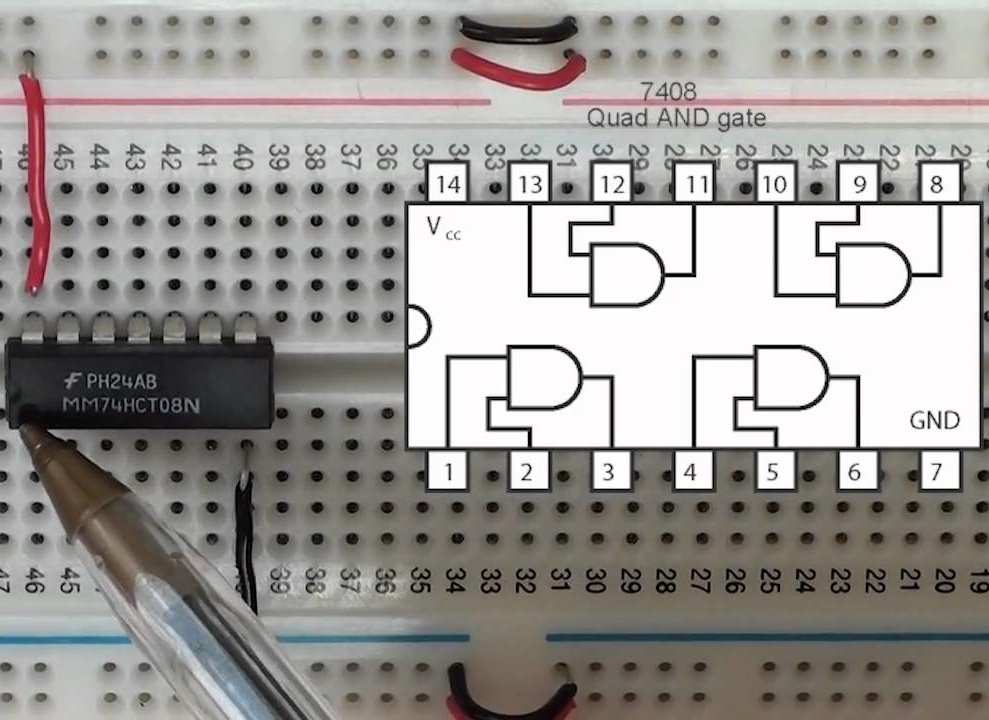
\includegraphics[height=0.4\textwidth]{images/logic_board_1.png}
        \hfil
        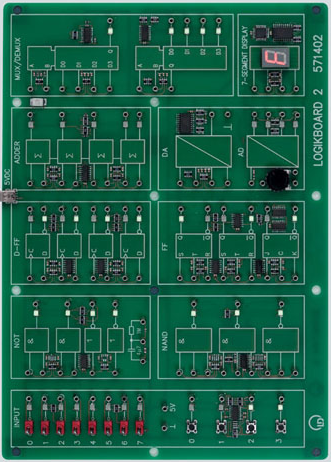
\includegraphics[height=0.4\textwidth]{images/logic_board_2.png}

    }
    \caption{Примеры плат и логических схем}
\end{figure}



%%========================
\paragraph{Анализ задачи.}
%%========================
Нам дан пример схемы с~логическими элементами. Нужно ответить на~следующие вопросы и сформулировать задачу.
\begin{enumerate}
    \item Какова предметная область?
    \begin{itemize}
        \item Работаем с~элементами математической логики.
    \end{itemize}

    \begin{figure}[h]
        {\centering
            \fbox{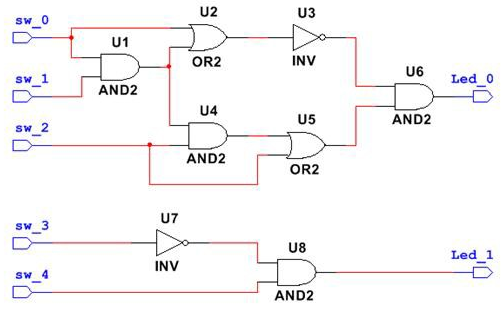
\includegraphics[width=0.35\textwidth]{images/logic_elements.png}}

        }
        \caption{Логические элементы}
        \label{fig:logicelems}
    \end{figure}

    \item В~каком контексте нужно разработать программный код?
    \begin{itemize}
        \item Необходим программный код, который позволяет смоделировать работу данной схемы.
        \item Этот код вполне вероятно будет использован для~моделирования подобных схем.
        \item Было бы удобно, если бы моделирование схемы не~зависело от~способа отображения процесса её работы (рисования).
    \end{itemize}

    \item Анализ исходных данных:
    \begin{itemize}
        \item На~схеме изображены не~все существующие логические элементы.
        \item На~схеме нет циклов.
        \item Есть логическое отрицание, но не~используются отрицания на~выходах/входах логических элементов.
    \end{itemize}
\end{enumerate}



%%=========================
\paragraph{Проектирование.}
%%=========================
Необходимо предусмотреть гибкость разрабатываемого программного кода.
\begin{itemize}
    \item Расширение функционала не~должно вынуждать полностью переписывать исходный код.
    \item Разделение на~небольшие части, подзадачи, которые могут быть использованы независимо (принцип <<разделяй и властвуй>>).
\end{itemize}

\bigskip Продумаем примеры того, как бы мы хотели видеть использование разработанного программного кода:
\begin{enumerate}
    \item Создание элементов.
    \begin{itemize}
        \item При~создании логического элемента нужно указать его тип (тип объекта), инвертирован ли его выход (по~умолчанию не~инвертирован), задать \code{callback}-функцию (по~умолчанию \code{nullptr}).
        \item При~создании источника логического значения (сигнала) нужно указать это значение (по~умолчанию \code{Signal::off}).
    \end{itemize}

    \item Соединение элементов.
    \begin{itemize}
        \item Соединений между логическими элементами гораздо больше, чем самих элементов.
        \item При~попытке сделать цикл в~схеме должно генерироваться исключение.
        \item Нужно предусмотреть (насколько это возможно) интуитивно понятный и лаконичный способ для~задания соединений.
        \item Удобно было бы соединять элементы по~цепочке.
        \item Будем использовать оператор \code{>>} для~соединения элементов (\code{and1 >> or2}).
        \item Подключение на~инвертированный вход вполне удобно смотрится с~использованием оператора~\code{\textasciitilde} (\code{or3 >> \textasciitilde{}and5}).
    \end{itemize}

    \item Изменение элементов.
    \begin{itemize}
        \item Для~задания логического значения источника удобно использовать оператор~\code{=} (\code{src1 = Signal::on}).
        \item Расчёт значений на~выходе каждого логического элемента должно происходить автоматически при~изменении состояния на~выходе элементов ниже по~цепочке.
        \item При~изменении состояния на~выходе элемента, этот элемент должен вызывать \code{callback}-функцию.
    \end{itemize}

    \item Получение значения на~выходе логического элемента.
    \begin{itemize}
        \item Оператор преобразования логического элемента в~значение \code{bool}.
    \end{itemize}
\end{enumerate}



%%============================
\paragraph{Первая реализация.}\label{par:logic:v1}
%%============================
Предлагаем самостоятельно разработать первую версию на~основе материала \textbookref{главы~9}.



%%================
\paragraph{P.\,S.}
%%================
Позже мы вернёмся к~проектированию классов для~моделирования схемы логических элементов, когда познакомимся с~наследованием и основами объектно-ориентированного программирования. Также мы добавим рисование элементов на~экране.



%%================
\WhatToReadSection
%%================
\textcite{Stroustrup:2016:ru}: \textbf{глава~10}



%%===============
\ExercisesSection
%%===============
\begin{exercise}
\item Выполните упражнения из~\textbookref{главы 9} учебника.

\end{exercise}
